\documentclass{bioinfo}
\copyrightyear{2016} \pubyear{2016}

\access{}%Advance Access Publication Date: Day Month Year}
\appnotes{}%Manuscript Category}

\begin{document}
\firstpage{1}

\subtitle{}%Database applications}

\title[POODLE]{POODLE 1.0 - To the core of your data}
\author[Ditz, Schroeder]{Jonas Ditz\,$^{\text{\sfb 1,}*}$ and Benjamin Schroeder\,$^{\text{\sfb 1,}*}$} 
\address{$^{\text{\sf 1}}$Department of Informatics, Eberhard Karls University, T\"ubingen, 72076, Germany.}

\corresp{$^\ast$To whom correspondence should be addressed.}

\history{}%Received on XXXXX; revised on XXXXX; accepted on XXXXX}

\editor{}%Associate Editor: XXXXXXX}


\abstract{\textbf{Motivation:} Many life science laboratories are still using Excel files to organize their data. 
	This leads to a huge workload for maintenance as well as a inconvenient access and update routine. 
	POODLE provides an easy-to-use and powerful interface to improve the cloning work of a lab.\\
\textbf{Results:} POODLE is a Java-based web interface, which allows intuitive access, update and 
manipulation of data for cloning.\\
\textbf{Contact:} \href{}{forename.surname@student.uni-tuebingen.de}\\
\textbf{Supplementary information:} Supplementary data and the code are available at \textit{https://github.com/derjedi/BioinformaticsI\-Assigments/tree/master/poodle\_project}
online.}

\maketitle

\section{Introduction}

\enlargethispage{12pt}
The POODLE project is a project which deals with really daily duty in a bio laboratory. Due to the data managment aspect of sequences and the task providing information fast, the project is clearly settled in the computer science field. The background data, which was obtained, was focussed on cloning for protein function studies or structure elucidation. Therefore we will focus on this application of the POODLE.
  
\subsection{A real world pipeline}
The cloning procedure is a standard strategy, which is used in nearly every life science lab. One possible application is in protein structure-function relationship studies. These studies use proteins, with a known sequence and start to modify the sequence with mutationsin order to observe changes  in the protein structure or functional bahaviour. The general pipeline of such an experiment could be, introducing the mutation via cloning, isolating the mutated protein and visualisation of differences via several methods. The visualisation for example could be an NMR interaction study or via X-Ray-Crystallography or any other essay. POODLE trys to manage the first  step of this pipeline, which is not only in this pieline the basic step.
\subsection{cloning as lab strategy}
Cloning is the key to a huge ammount of variety in the resulting protein constructs. Via cloning, it is possible to remove a function, add a function to a protein or influence the structure. Today, there are many different cloning methods available, like the classical restriction approach, the site directed mutagenisis method, restriction free cloning or the Crisp-Cas system. All mehtods have a specific task and are chosen in various situation. For this paper we want to stick to the site directed mutagenisis, which was initially developed by stratagene as QuickChange site-directed mutagensis kit. This method allow to introduce small directed mutation into a protein on DNA level. these mutations can be used to perform point mutations or switch single or multiple amino acids.

\begin{figure}
	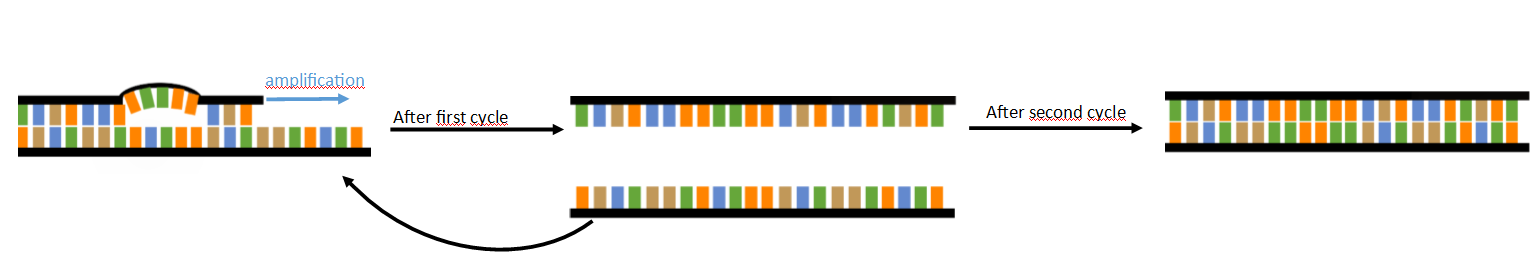
\includegraphics[width=0.4\textwidth]{"../Documents/img/QC-cloning.png}
	\caption{Schema of QC}
	\label{QC-pic}
\end{figure}

\subsection{cloning methods}
Classsic Cloning, Quickchange, Restriction free cloning

\subsection{The resulting data}
primer
cloningVectors
proteinConstructs


\section{Approach}

As already mentioned above many life-science laboratories use Excel files for storing and working with 
data. But Excel files have a few drawbacks, which make working with them inconvenient. One of the 
biggest problems occurs, if more than one member of the laboratory tries to access the file at the 
same time. Inconsistent files can be the result of a simultaneous access. Second, searching in a Excel file is not as easy as 
it could be. Furthermore, licenses for Excel are expensive and switching to a free software solution 
saves a lot of money. The reason for using Excel rather than a database system is that most life-scientist 
are not familiar with database systems and prefer the GUI of Excel to work with. We are 
trying to solve that problem by combining the functionality of a database system with an intuitive and 
easy-to-learn handling.

\begin{methods}
\section{Methods}

POODLE is build as a two-layer software. The first layer consists of the database and routines to 
automatically build and update that database. The second layer consists of the web service that is 
used to access, update and manipulate data. This is the front end layer and provides access to all 
functions for the user, such as accessing the database, manipulating data and using the in-build 
Blast functionality.

\subsection{Database layer}

SQLite\footnote{http://www.sqlite.org/} is the database system running in the background. We chose 
this software for several reasons. First, it is free of charge. Second, and more important SQLite is 
a small and fast database system written in C. Since, the whole database is stored just in one file
SQLite has a incredibly good performance combined with a really small among of required space. And there 
is the possibility to create a mobile version of POODLE without changing the whole database system, 
which may be interesting in the future. Besides, 
SQLite guaranties that transactions have all ACID (Atomicity, Consistency, Isolation and Durability) properties even if a system crash or power failure occurs. So 
we have a robust storage and access of data as well as a lot of functionality provided by the database 
system. In addition to the SQLite database POODLE's software creates a BLAST database for the provided 
data, too. 

The build and update process is implemented in Python. POODLE combines a SQL database with several 
local Blast databases and this routine 
ensures that the SQLite database and BLAST databases are always in the same state. 
It also makes the database a little bit safer, since changes can be reviewed before inserting them 
into the database. Furthermore, the user does not need detailed knowledge about SQL to create the 
database, which may be helpful for many laboratories.

\subsection{Web service}

POODLE web service is build with Vaadin\footnote{https://vaadin.com/home}. We chose that framework 
because it allows a safe 
communication between the front end and the database layer as well as a smooth and intuitive user 
interface. Since a website developed with Vaadin is highly modular, it is easy to extend the web 
service in the future. That could be necessary, if new functionalities are required. Currently, 
there are three pages with different roles. The search page provides a formula that can be used 
to perform a simple SQL search in the local database. Therefor, different fields are displayed and 
can be filled by the user. A click on the search button will automatically build a SQL query and 
results are displayed, if there are available results. The new entry page allows to insert a new 
entry into the database. It also provide a Blast search against the NCBI databases to check, whether 
there are already available information about the new sequence or not. Last but not least, users can 
perform a local Blast search against their one database or a remote Blast search against the NCBI 
databases on the Blast page. That functionality can be found on the Blast page. 

\subsection{Blast functionality}

Our software package provides not just a database functionality for powerful and safe data storage 
and an easy-to-use interface but also a Blast (\citealp{Altschul01}) functionality. This function 
is implemented by using a combination of Blast binaries provided by NCBI and the Biojava Api 
(\citealp{Prlic01}). There are two different Blast searches available in POODLE. On one hand, there 
is a remote Blast search on the NCBI server. And on the other hand, there is a local Blast search. 
The remote Blast search is not a fully functional copy of the NCBI web service but can be used to 
perform a quick and simple search against databases provided by NCBI, e.g. Swissprot (\citealp{Donavan01}). But we 
do not recommend to overuse that because too many requests may cause a blacklisting by NCBI. This 
remote Blast routine is mainly for the insertion of a new entry. The idea is to check whether there 
are information about the new sequence. But it can also used separated from the new entry routine. 
The local Blast routine does everything someone would 
expect from a Blast search but against the local database, hence local Blast. There a several programs, 
e.g. blastn or blastp, available for both Blast methods. 

\end{methods}

%\begin{figure}[!tpb]%figure1
%\fboxsep=0pt\colorbox{gray}{\begin{minipage}[t]{235pt} \vbox to 100pt{\vfill\hbox to
%235pt{\hfill\fontsize{24pt}{24pt}\selectfont FPO\hfill}\vfill}
%\end{minipage}}
%\centerline{\includegraphics{fig01.eps}}
%\caption{Caption, caption.}\label{fig:01}
%\end{figure}

%\begin{figure}[!tpb]%figure2
%%\centerline{\includegraphics{fig02.eps}}
%\caption{Caption, caption.}\label{fig:02}
%\end{figure}


\section{Discussion}

POODLE is completely open-source. So the user can adapt the code at any point of the software. To make 
this adaption as easy as possible for the user we chose to use widely known software inside of POODLE. 
Most scientist have heard of SQL as a database managment system. So it is not too venture to assume 
that there are people with basic SQL knowledge in most of the laboratories. And that means these 
laboratories do not have to use POODLE as a black box. We chose SQLite over all other SQL databases 
for the reasons described in the method section. 

The build up process of the database is written in Python. There are two reasons for that. First, 
Python is an easy and powerful language which makes it possible for the user to adapt the build up 
process without detailed programming knowledge. And second Python2.7 is a default package of most 
operating systems installed on a server. We tried to make POODLE as platform independent as possible 
and that helps to reach our goal.

Vaadin was chosen as the running framework for several reasons. Java is a widely used programming language 
in the scientific world. So there is a relative high chance for a person in the laboratory, who 
is able to work with
Java. Again we want to make adaption as easy as possible for the user. Furthermore, Vaadin needs a 
tomcat server. Such a server is provided free of charge by Apache\footnote{http://www.apache.org/}. 
So the user does not have to face extra charges just to be able to use POODLE. More reasons for 
Vaadin are discussed above.

\section{Conclusion}

POODLE provides a safe storage of cloning data as well as a easy-to-use interface for 
interacting with these data. Besides, it comes with functionalities like local and remote Blast 
search that can improve the workflow during cloning. 

It is our goal to improve the software in the future by adding new functionalities like a chromatogram 
viewer and the possibility to add annotations to sequences. 

\section*{Acknowledgements}

We would like to thank Silke Wiesner and her group at the Max-Plack-Institute for Developmental Biology 
in T\"{u}bingen for providing us with real-world data and fruitful discussions.

\section*{Funding}

This work has been supported by ... nobody. Seriously, not anybody. We know that is sad but it is hard 
to convince people giving their money away.

%\bibliographystyle{natbib}
%\bibliographystyle{achemnat}
%\bibliographystyle{plainnat}
%\bibliographystyle{abbrv}
%\bibliographystyle{bioinformatics}
%
%\bibliographystyle{plain}
%
%\bibliography{Document}


\begin{thebibliography}{}

\bibitem[Altschul {\it et~al}., 1990]{Altschul01}
Altschul, S.F., Gish, W., Miller, W., Myers, E.W., Lipman, D.J. (1990) Basic local alignment search tool., {\it J. Mol. Biol.}, {\bf 215}, 403-410.

\bibitem[Prli\'{c} {\it et~al}., 2012]{Prlic01}
Prli\'{c}, A., Yates, A., Bliven, S. E., Rose, P. W., Jacobsen, J., Troshin, P. V., ... Willis, S. (2012) BioJava: an open-source framework for bioinformatics in 2012. {\it Bioinformatics}, {\bf 28}(20), 2693-2695. http://doi.org/10.1093/bioinformatics/bts494

\bibitem[O'Donavan {\it et~al}., 2002]{Donavan01}
O'Donovan, C., Martin, M.J., Gattiker, A., Gasteiger, E., Bairoch, A., Apweiler, R. (2002) High-quality protein knowledge resource: SWISS-PROT and TrEMBL {\it Brief. Bioinform.}  {\bf 3} (3), 275-284. doi: 10.1093/bib/3.3.275 

\bibitem[Alberts {\it et~al}., 2002]{Alberts01}
Alberts B, Johnson A, Lewis J, et al. (2002) Molecular Biology of the Cell. 4th edition. {\it New York: Garland Science}. Studying Gene Expression and Function. Available from: http://www.ncbi.nlm.nih.gov/books/NBK26818/

\end{thebibliography}
\end{document}
